%%This is a very basic article template.
%%There is just one section and two subsections.
\documentclass{article}
\usepackage{graphicx}
\usepackage{cite}
\usepackage{booktabs}
\graphicspath{ {images/} }


\begin{document}

\bibliographystyle{plain}


\section{Title}

\subsection{Introduction}
%introduce whole study and paper here (together)

\subsection{Background}
%literature background (Natalie)

\subsection{Materials and Methods}


The original dataset utilised in this study consists in 1,562 responses from a
quantitative survey conducted on behalf of the ACNC by ChantLink in 2013. It
does not include a pilot phase of 62 responses. The survey collected information
about levels of trust in charities and factors that may affect these levels. The
respondents were asked to rate their level of trust and their agreement with a
series of statements about charities on a scale from 1 to 10. They also were
asked about their involvement, knowledge of charities sector and demographics.
Specifically, the survey was divided into 5 sections: Awareness and Involvement
in Charities, Trust, Regulation, Public Register of Charities and Demographics.

Aiming to cluster the survey respondents according their trust and confidence in
charities, a new dataset was obtained from the original dataset. It consists of
the Trust section responses, which were rated on the scale from 1 to 10. In
addition, the questions not answered by all the respondents and those with
user-typed responses were removed. This procedure was adopted in order to select
informative and comparable questions as the survey contains different types of
questions. Overall, 1,562 responses of 43 different questions was considered in
the clustering step.

Since the dataset can be represented as a graph, the methodology utilised for
clustering is based on a novel graph-based clustering algorithm propose by
~\cite{Inostroza2008}. The MSTkNN combines a Minimum Spanning Tree (MST) and a
k-Nearest Neighbor (kNN) proximity graphs. This combination allows us to perform
a graph partitioning operation, which produces a clustering of the dataset
represented by its graph. The graph partitioning separates the data in groups
with similar characteristics utilizing a given proximity measurement. In this
case, the Spearman correlation was used to measure the distance between
different features of the dataset's graph.

Given a undirected and connected graph, a MST is a subgraph which is a tree and
contain all the objects connected by the minimum possible distance between each
other, based on a determined measurement of the distance. Whereas, the kNN graph
is a graph where their objects are connected if they are commutual k nearest
neighbors of each other according to a defined value of k. In this work, the
value of k was defined as 3 for computing the kNN graph. The merge of these
methods permit delete the connection between two objects in the MST if they are
not reciprocally one of the k nearest of each other. Consequently, the MST is
partitioned into smaller subgraphs, which are the resultant clusters.

%Normalization by row?

After clustering the dataset, the new score introduced by~\cite{Marsden2013}
was computed to highlight the individual characteristics of each cluster. The
CM1 score gives a overview about differences in averages for each feature from
a specific cluster in the investigated dataset. The rank of the CM1 scores of a
cluster can be split into top or bottom features. The top features refers to
features whose average are greater in a specific cluster than in all the others,
while bottom refers to features whose average are less in a specific cluster
than in all the others. The CM1 scores are then computed using the following
formula~(\ref{eq:01}).

\begin{equation}
CM1(w,X,Y) = \frac{\frac{1}{\left|X\right|}  \sum_{x \in X} x_{w} - \frac{1}{\left|Y\right|}  \sum_{y \in Y} y_{w}} {1 + max_{y \in Y } \left\{ y_{w} \right\}- min_{y \in Y} \left\{y_{w}\right\} } \label{eq:01}
\end{equation}

%this study was based on the study done in UK and NZ


\subsection{Results}

The MSTkNN clustering algorithm was able to find 7 different clusters of
different sizes according Figure \ref{fig:Clusters}. These included Cluster0
with 195 respondents (13\%), Cluster1 with 157 (10\%), Cluster2 with 192 (12\%),
Cluster3 with 317 (20\%), Cluster4 with 45 (3\%), Cluster5 with 556 (36\%) and
Cluster6 with 100 (6\%).


\begin{figure}[h]
	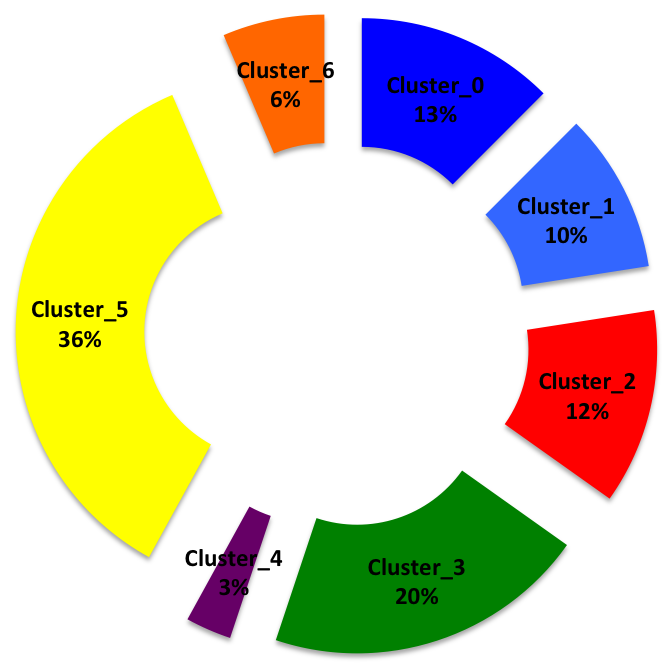
\includegraphics[scale=0.5]{Clusters.png}
	\caption{Distribution of respondents among 7 different clusters obtained
	by MSTkNN clustering algorithm.}
	\label{fig:Clusters}
\end{figure}

The CM1 score was then calculated for all the 43 features of the new dataset
for each of the discovered clusters. The selected top and bottom features for
each cluster is presented in the Tables~\ref{tab:bottom} and~\ref{tab:top}.
These tables present the CM1 scores in descending order. The Bottom features
contain the most negative ranked features while the top features contain the
most positive ranked features for each cluster. In this context, the bottom
features highlight the questions with the lowest rates for a specific cluster
compared to others. However, the top features highlight the questions with the
highest rates for a selected cluster compared to others.	

\begin{table}[htbp]
  \centering
  \caption{Bottom features for each cluster (presented in ascending order of
  score)}
    \begin{tabular}{rrrrrrr}
    \toprule
    Cluster\_0 & Cluster\_1 & Cluster\_2 & Cluster\_3 & Cluster\_4 & Cluster\_5 & Cluster6 \\
    \midrule
    Q7B\_7 & Q9\_13 & Q9\_10 & Q11\_6\_1 & Q9\_15 & Q9\_07 & Q11\_1\_1 \\
    Q7B\_11 & Q9\_14 & Q9\_02 & Q11\_5\_1 & Q9\_04 & Q9\_05 & Q11\_5\_1 \\
    Q7B\_9 & Q9\_19 & Q7B\_7 & Q11\_1\_1 & Q9\_16 & Q9\_06 & Q11\_4\_1 \\
    Q7B\_6 & Q9\_10 & Q7B\_6 & Q11\_3\_1 & Q9\_21 & Q9\_20 & Q11\_6\_1 \\
    Q7B\_5 & Q9\_03 & Q9\_03 & Q11\_2\_1 & Q9\_24 & Q9\_21 & Q11\_2\_1 \\
    Q7B\_10 & Q9\_11 & Q9\_23 & Q9\_15 & Q7B\_1 & Q11\_5\_1 & Q11\_3\_1 \\
    Q7B\_3 & Q9\_09 & Q7B\_11 & Q9\_04 & Q9\_25 & Q11\_3\_1 & Q9\_15 \\
    Q9\_09 & Q9\_01 & Q9\_25 &       & Q9\_23 &       & Q9\_04 \\
    Q9\_02 & Q7A   & Q9\_19 &       & Q7B\_2 &       &  \\
    Q9\_10 & Q9\_12 & Q9\_22 &       & Q9\_20 &       &  \\
    Q7B\_4 & Q9\_18 & Q7A   &       & Q9\_22 &       &  \\
    Q7B\_8 & Q9\_23 & Q9\_24 &       &       &       &  \\
          &       & Q9\_08 &       &       &       &  \\
    \bottomrule
    \end{tabular}
  \label{tab:bottom}
\end{table}

\begin{table}[htbp]
  \centering
  \caption{Top features for each cluster (presented in descending order of
  score)}
    \begin{tabular}{rrrrrrr}
    \toprule
    Cluster\_0 & Cluster\_1 & Cluster\_2 & Cluster\_3 & Cluster\_4 & Cluster\_5 & Cluster6 \\
    \midrule
    Q9\_21 & Q9\_07 & Q9\_07 & Q9\_02 & Q11\_5\_1 & Q9\_14 & Q7B\_4 \\
    Q9\_23 & Q9\_06 & Q9\_05 & Q9\_10 & Q11\_4\_1 & Q9\_13 & Q7B\_6 \\
    Q9\_20 & Q9\_05 & Q9\_06 & Q9\_09 & Q11\_1\_1 & Q9\_19 & Q7B\_11 \\
    Q9\_24 & Q9\_21 & Q11\_5\_1 & Q7B\_7 & Q9\_10 & Q9\_03 & Q7B\_3 \\
    Q11\_5\_1 & Q9\_20 & Q11\_3\_1 & Q7B\_11 & Q9\_02 & Q9\_11 & Q9\_02 \\
    Q9\_06 & Q11\_5\_1 & Q11\_6\_1 & Q7A   & Q7B\_3 & Q9\_16 & Q7B\_7 \\
    Q11\_3\_1 & Q11\_3\_1 & Q9\_21 & Q9\_03 & Q11\_2\_1 & Q9\_01 & Q7B\_5 \\
    Q9\_05 & Q11\_6\_1 & Q9\_20 & Q9\_19 & Q7B\_4 & Q9\_08 & Q7B\_2 \\
    Q9\_22 & Q11\_1\_1 & Q11\_1\_1 &       &       & Q9\_12 & Q7B\_10 \\
    Q9\_25 & Q11\_2\_1 & Q11\_4\_1 &       &       &       & Q9\_10 \\
    Q11\_6\_1 & Q11\_4\_1 &       &       &       &       & Q7B\_8 \\
    Q9\_07 &       &       &       &       &       & Q7B\_9 \\
    Q11\_1\_1 &       &       &       &       &       & Q7B\_1 \\
    \bottomrule
    \end{tabular}
  \label{tab:top}
\end{table}

% Cluster 0

The Figure~\ref{fig:CM1Cluster0} demonstrate the CM1 score for the 43 features
for Cluster0, with the 12 bottom and 13 top features shown in red and green
respectively, as presented in Tables~\ref{tab:bottom} and~\ref{tab:top}. The
question Q7B, which aims to rate the trust and confidence levels between
different institutions and organizations, is shown to dominate among the bottom
features. It indicates a lower level of trust and confidence in these
institutions and organizations. Furthermore, it is a distinctly characteristic
for this cluster as observed in Table~\ref{tab:bottom}. The difference between
the cumulative CM1 scores for the top and bottom features for Cluster0 is shown
in the Figure~\ref{fig:DifferencesCluster0}. It is observed that this cluster
score higher positive results against these features.


\begin{figure}[h]
	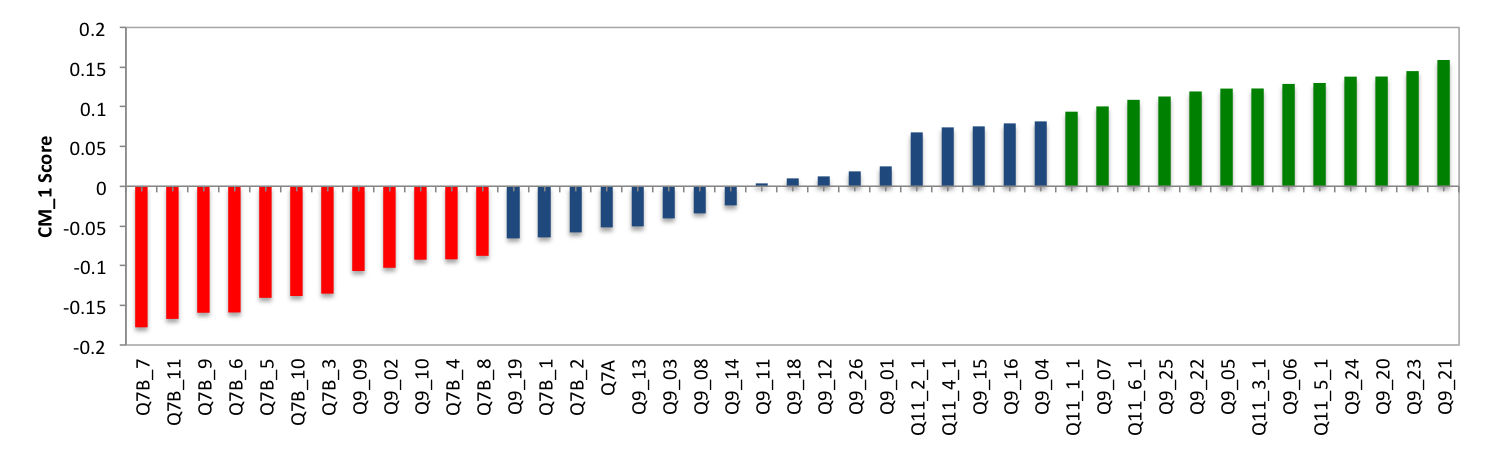
\includegraphics[ width=\textwidth ]{CM1_Cluster0.png}
	\caption{CM1 Scores for the 43 features for Cluster0, based on the new dataset.
	The selected top and bottom features are shown in red and green respectively
	and are presented in Tables~\ref{tab:bottom} and~\ref{tab:top}. The majority of
	bottom features are from question Q7B which suggests lower rates of trust and
	confidence in specific institutions and organizations.}
	\label{fig:CM1Cluster0}
\end{figure}
\begin{figure}[h]
	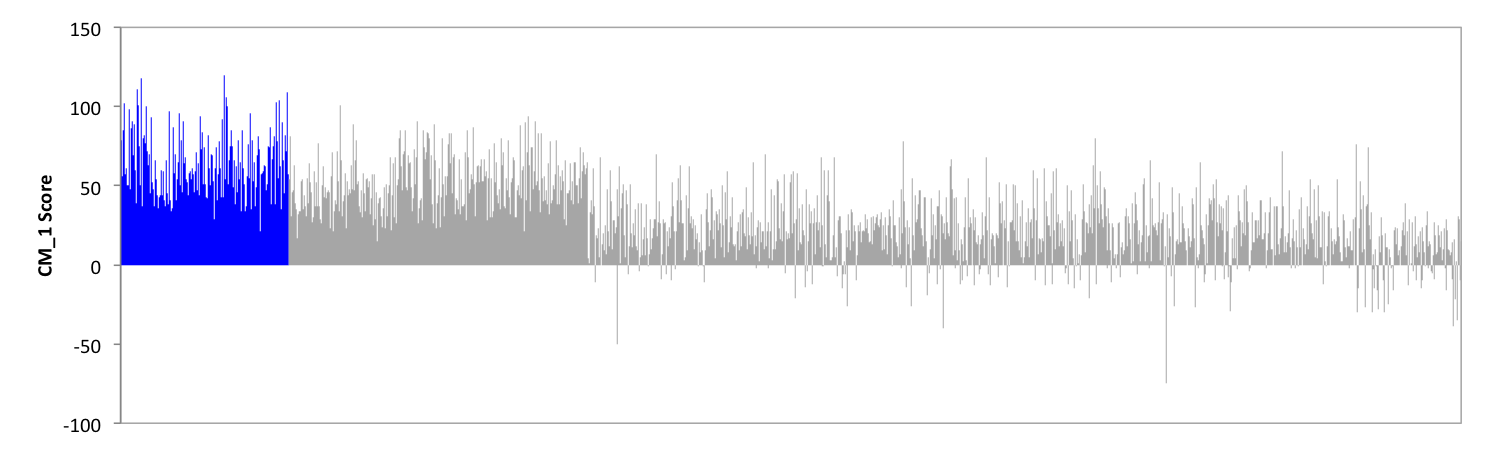
\includegraphics[ width=\textwidth]{Difference_Cluster0.png}
	\caption{Difference between the cumulative CM1 scores for the 12 bottom and 13
	top features for Cluster0, as presented in Tables~\ref{tab:bottom}
	and~\ref{tab:top}. The respondents of Cluster0 are shown in blue. It is
	observed that they score higher positive results against these features.}
	\label{fig:DifferencesCluster0}
\end{figure}

% Cluster 1 and Cluster 2

The 12 bottom and 11 top CM1 scores for the 43 features for Cluster1 are shown
in Figure~\ref{fig:CM1Cluster1}, and the 13 bottom and 11 top CM1 scores for
Cluster2 are shown in Figure~\ref{fig:CM1Cluster2} in red and green
respectively. The top features of both clusters are mainly composed for the same
questions, Q9 and Q11, as observed in Table ~\ref{tab:top}. However they differ
among the bottom features. The presence of bottom features from question Q7 in
Cluster2 suggests a lower level of trust and confidence for this cluster. The
difference between cumulative CM1 scores for these top and bottom features for
Cluster1 and Cluster2 are shown in the Figures~\ref{fig:DifferencesCluster1}
and~\ref{fig:DifferencesCluster2} respectively. It is observed that these
clusters score positive results against these features and also score relatively
close results although they differ among the top features.

\begin{figure}[h] %% Cluster1
	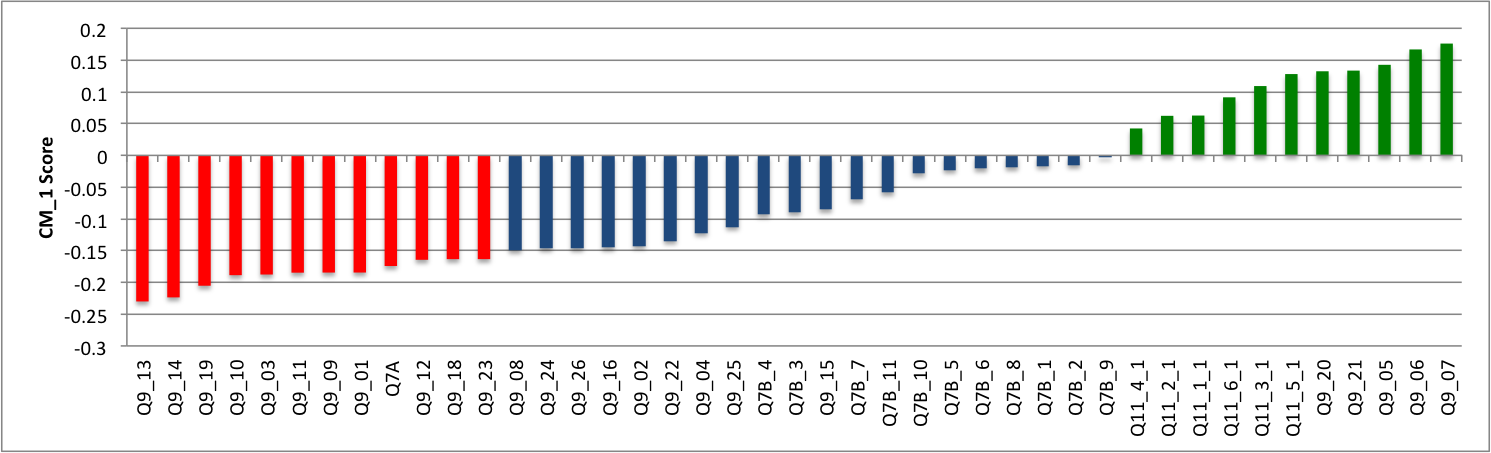
\includegraphics[ width=\textwidth ]{CM1_Cluster1.png}
	\caption{CM1 Scores for the 43 features for Cluster1, based on the new dataset.
	The selected top and bottom features are shown in red and green respectively
	and are presented in Tables~\ref{tab:bottom} and~\ref{tab:top}. The presence of
	question Q11 among the top features suggests that the respondents from this
	group a great care about the information that charities may provide.}
	\label{fig:CM1Cluster1}
\end{figure}
\begin{figure}[h]
	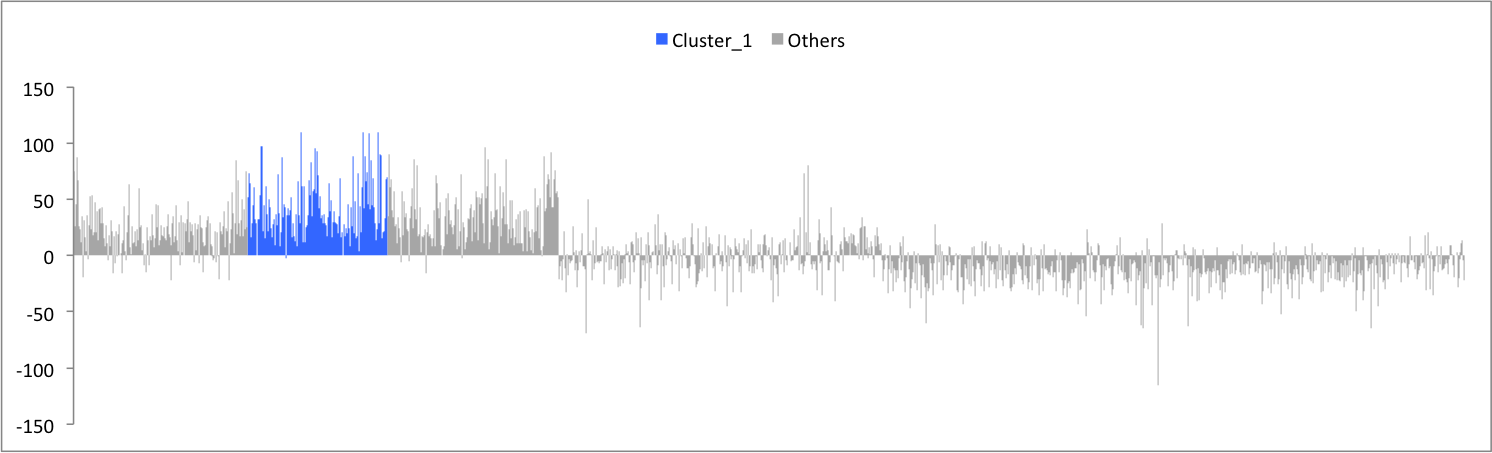
\includegraphics[ width=\textwidth]{Difference_Cluster1.png}
	\caption{Difference between the cumulative CM1 scores for the 12 bottom and 13
	top features for Cluster1, as presented in Tables~\ref{tab:bottom}
	and~\ref{tab:top}. The respondents of Cluster1 are shown in light blue. It is
	observed that they score higher results against these features.}
	\label{fig:DifferencesCluster1}
\end{figure}

\begin{figure}[h] %% Cluster2
	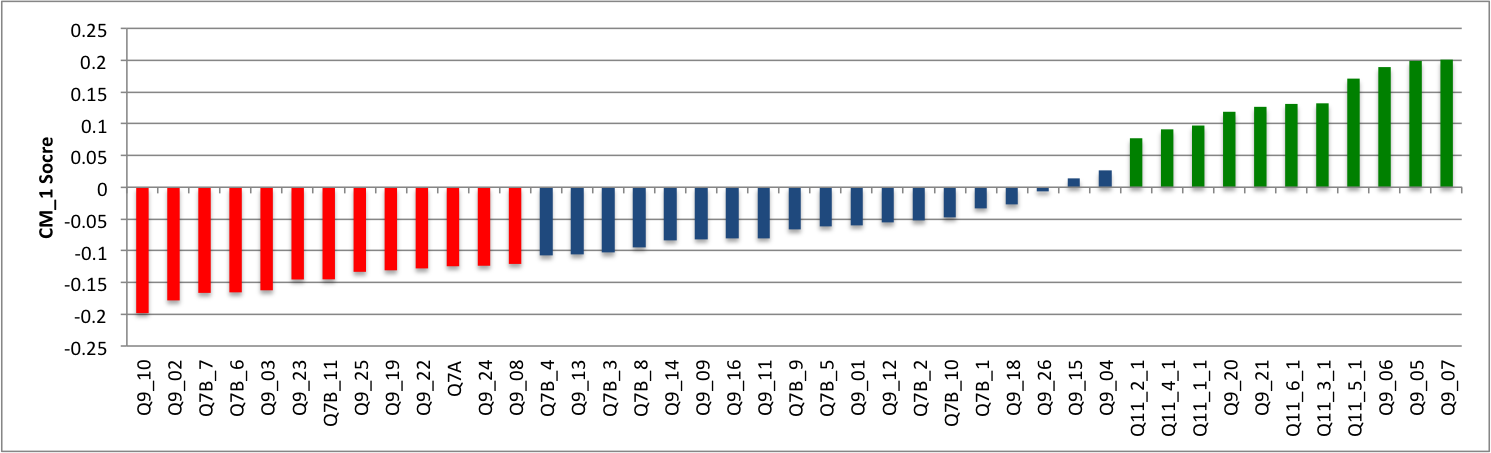
\includegraphics[ width=\textwidth ]{CM1_Cluster2.png}
	\caption{CM1 Scores for the 43 features for Cluster2, based on the new dataset.
	The selected top and bottom features are shown in red and green respectively
	and are presented in Tables~\ref{tab:bottom} and~\ref{tab:top}. The features
	from questions Q7B and Q7A among the bottom features suggests a low rate
	of trust and confidence. On the other hand, The top question Q11 suggests a
	greater concern about the information disponibilizide by charities.}
	\label{fig:CM1Cluster2}
\end{figure}
\begin{figure}[h]
	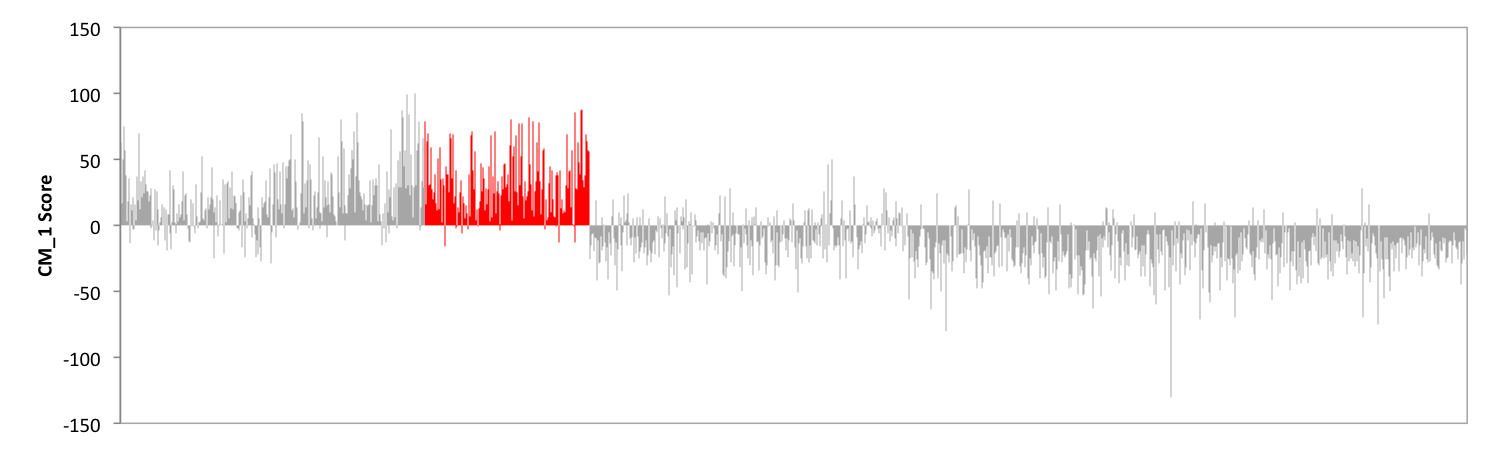
\includegraphics[ width=\textwidth]{Difference_Cluster2.png}
	\caption{Difference between the cumulative CM1 scores for the 13 bottom and 11
	top features for Cluster2, as presented in Tables~\ref{tab:bottom}
	and~\ref{tab:top}. The respondents of Cluster2 are shown in red. It is
	observed that they score higher results against these features and are
	relatively close from the respondents of Cluster1.}
	\label{fig:DifferencesCluster2}
\end{figure}

% Cluster 3

Figure~\ref{fig:CM1Cluster3} shows the 7 bottom and 8 top features for Cluster3
in red and green respectively. The Q11 features appear as the most negative
ranked features for this cluster. It suggests a very lower concern about the
information that charities may provide. The question Q7A is observed as a top
feature, and this question is only present in this cluster as a top feature. It
demonstrates a higher trust and confidence rate in Australian charities overall.
The difference between the cumulative CM1 scores for the top and bottom features
are shown in Figure~\ref{fig:DifferencesCluster3}. The respondents of Cluster3
score less negative results against these features.

\begin{figure}[h]
	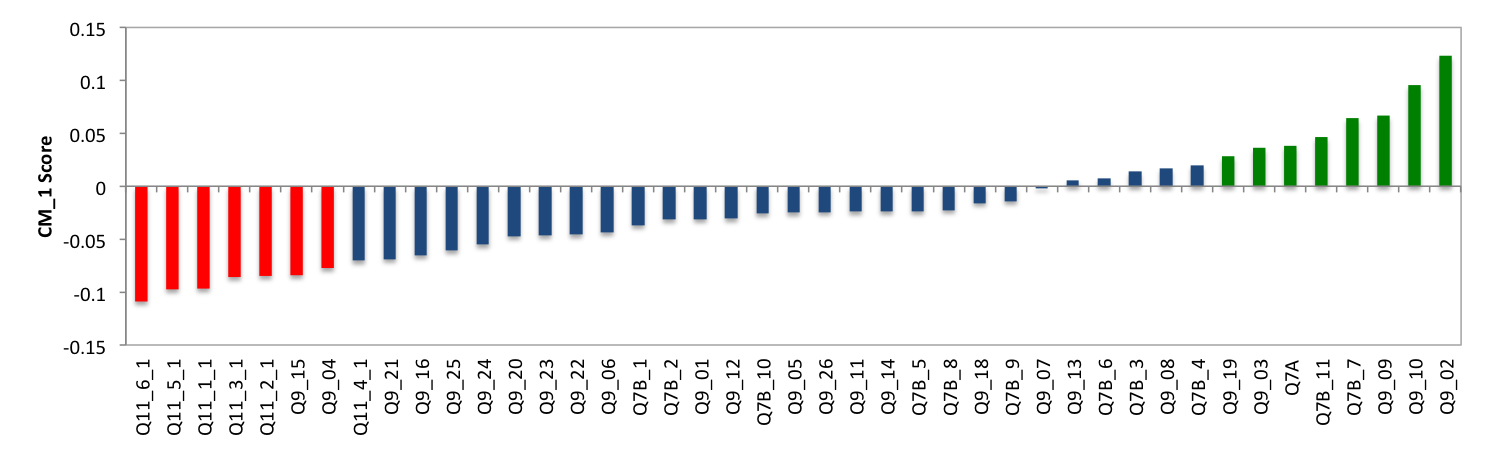
\includegraphics[ width=\textwidth ]{CM1_Cluster3.png}
	\caption{CM1 Scores for the 43 features for Cluster3, based on the new dataset.
	The selected top and bottom features are shown in red and green respectively
	and are presented in Tables~\ref{tab:bottom} and~\ref{tab:top}. The
	most negative ranked features are from question Q11 that suggests a low
	interest in the information that charities may provide. Additionally, the
	questions Q7A and Q7B among the most positive ranked questions indicate a
	higher rate of trust and confidence in charities.}
	\label{fig:CM1Cluster3}
\end{figure}
\begin{figure}[h]
	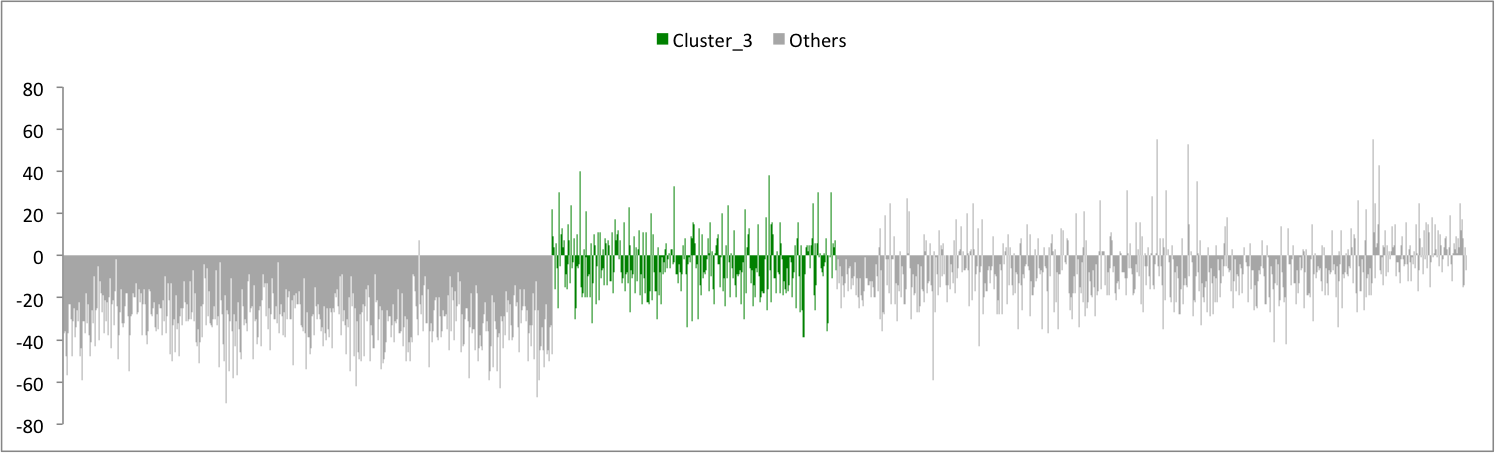
\includegraphics[ width=\textwidth]{Difference_Cluster3.png}
	\caption{Difference between the cumulative CM1 scores for the 7 bottom and 8
	top features for Cluster3, as presented in Tables~\ref{tab:bottom}
	and~\ref{tab:top}. The respondents of Cluster3 are shown in green. It is
	observed that they score less negative results against these features.}
	\label{fig:DifferencesCluster3}
\end{figure}


% Cluster 4

The Figure~\ref{fig:CM1Cluster4} demonstrate the CM1 score for the 43 features
for Cluster4, with the 11 bottom and 8 top features shown in red and green
respectively. The question Q9 dominate as a bottom feature while the question
Q11 as a to feature. The question Q11 among the top features suggests a greater
concern about the information provided by charities. The difference between the
cumulative CM1 scores for the top and bottom features for Cluster0 is shown in
the Figure~\ref{fig:DifferencesCluster4}. It is observed that the respondents of
Cluster4 score less negative results against these features.

\begin{figure}[h]
	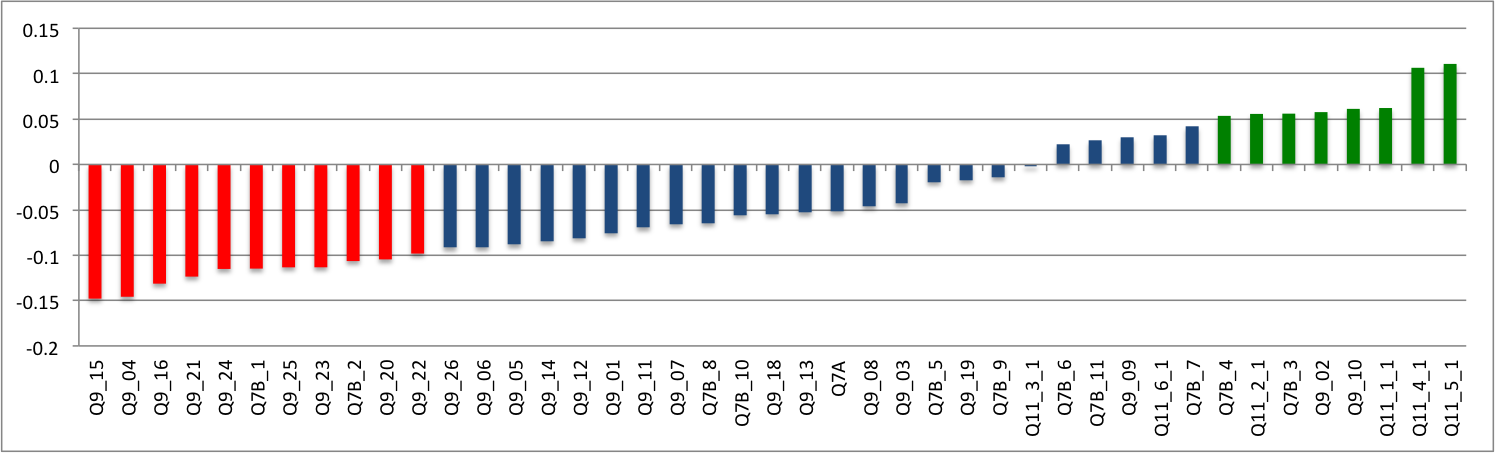
\includegraphics[ width=\textwidth ]{CM1_Cluster4.png}
	\caption{CM1 Scores for the 43 features for Cluster4, based on the new dataset.
	The selected top and bottom features are shown in red and green respectively
	and are presented in Tables~\ref{tab:bottom} and~\ref{tab:top}. The bottom
	features for Cluster4 consist mostly of Q9 features, and the top features
	consist of the questions Q7B, Q11 and Q9 features.}
	\label{fig:CM1Cluster4}
\end{figure}
\begin{figure}[h]
	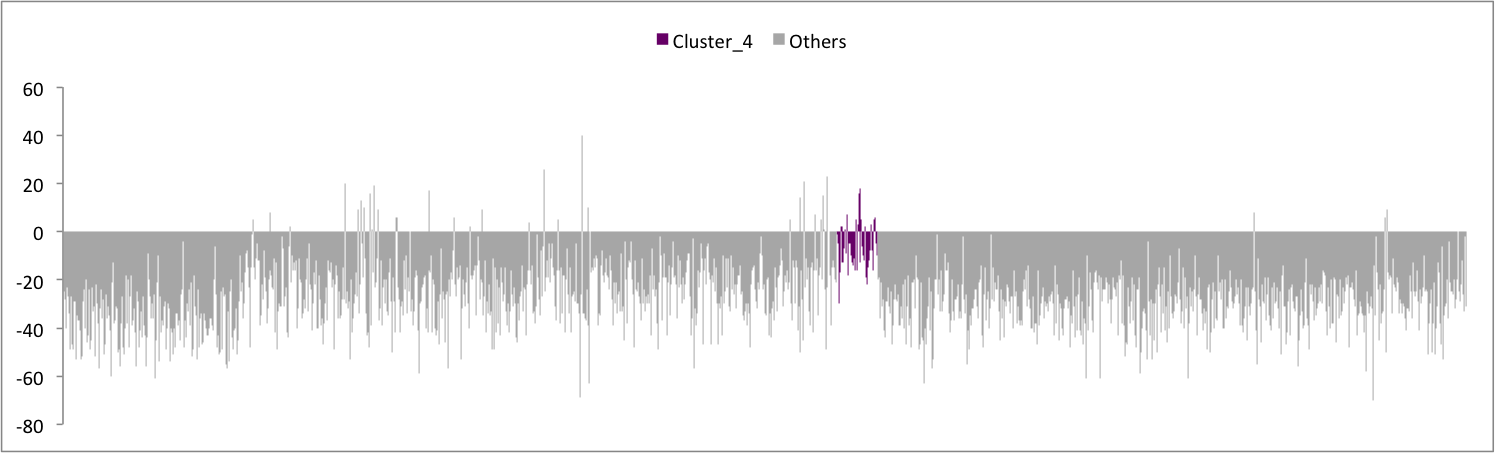
\includegraphics[ width=\textwidth]{Difference_Cluster4.png}
	\caption{Difference between the cumulative CM1 scores for the 11 bottom and 8
	top features for Cluster4, as presented in Tables~\ref{tab:bottom}
	and~\ref{tab:top}. The respondents of Cluster4 are shown in dark purple. It is
	observed that they score less negative results against these features}
	\label{fig:DifferencesCluster4}
\end{figure}

% Cluster 5

Figure~\ref{fig:CM1Cluster5} shows the 7 bottom and 9 top features for Cluster5
in red and green respectively. The Q9 question is the most ranked question in
both, bottom and top features. This fact might highlight important factors that
affect trust and confidence since the Cluster5 is the biggest cluster,
representing 36\% of all respondents. The difference between the
cumulative CM1 scores for the top and bottom features are shown in
Figure~\ref{fig:DifferencesCluster5}. It is observed that the respondents of
Cluster5 score strong positive results against these features.

\begin{figure}[h]
	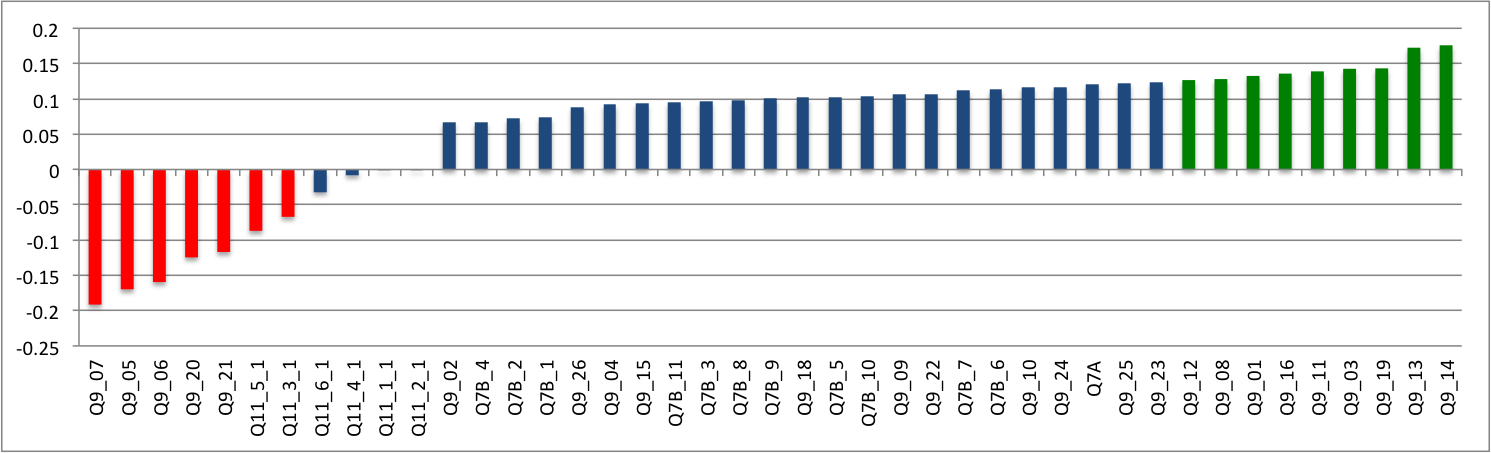
\includegraphics[ width=\textwidth ]{CM1_Cluster5.png}
	\caption{CM1 Scores for the 43 features for Cluster5, based on the new dataset.
	The selected top and bottom features are shown in red and green respectively
	and are presented in Tables~\ref{tab:bottom} and~\ref{tab:top}. Since
	Cluster5 is the biggest cluster and the question Q9 represents the most ranked
	bottom and top features, may it help to identify important factors that
	influence the trust and confidence rate.}
	\label{fig:CM1Cluster5}
\end{figure}
\begin{figure}[h]
	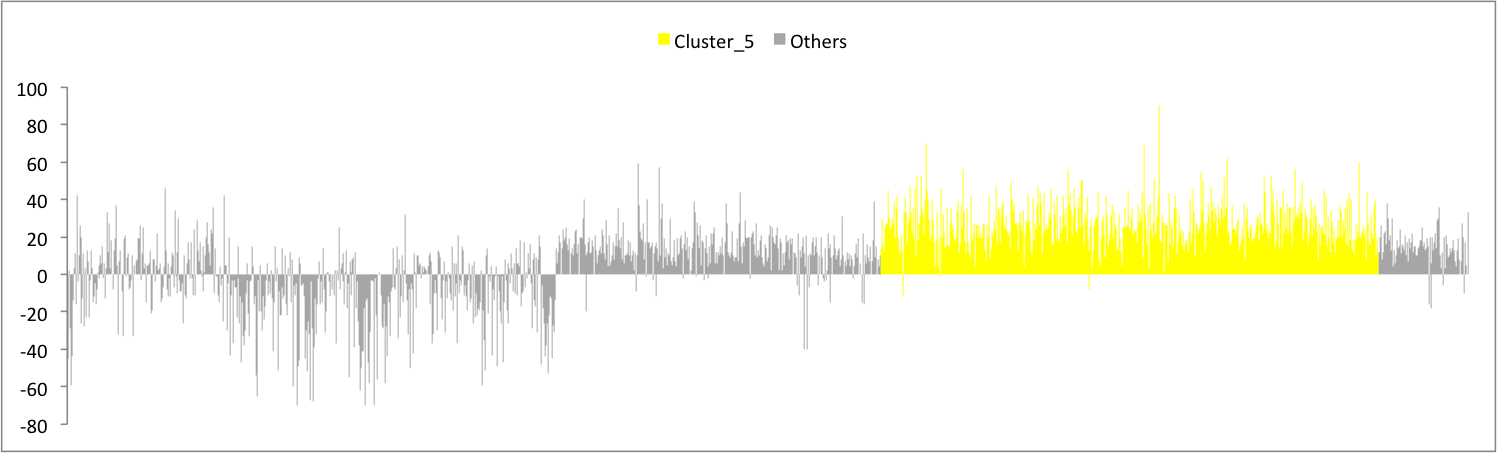
\includegraphics[ width=\textwidth]{Difference_Cluster5.png}
	\caption{Difference between the cumulative CM1 scores for the 7 bottom and 9
	top features for Cluster5, as presented in Tables~\ref{tab:bottom}
	and~\ref{tab:top}. The respondents of Cluster5 are shown in yellow. It is
	observed that they score strong positive results against these features}
	\label{fig:DifferencesCluster5}
\end{figure}

% Cluster 6

Figure~\ref{fig:CM1Cluster6} shows the 8 bottom and 13 top features for Cluster6
in red and green respectively. The Q11 question is the most ranked
bottom feature, which suggest a low concern about the information provided by
charities. Among the top features the most ranked question is Q7B, which
indicate a higher trust and confidence rate for this cluster. The difference
between the cumulative CM1 scores for the top and bottom features are shown in
Figure~\ref{fig:DifferencesCluster6}. It is observed that the respondents of
Cluster6 score strong positive results against these features.

\begin{figure}[h]
	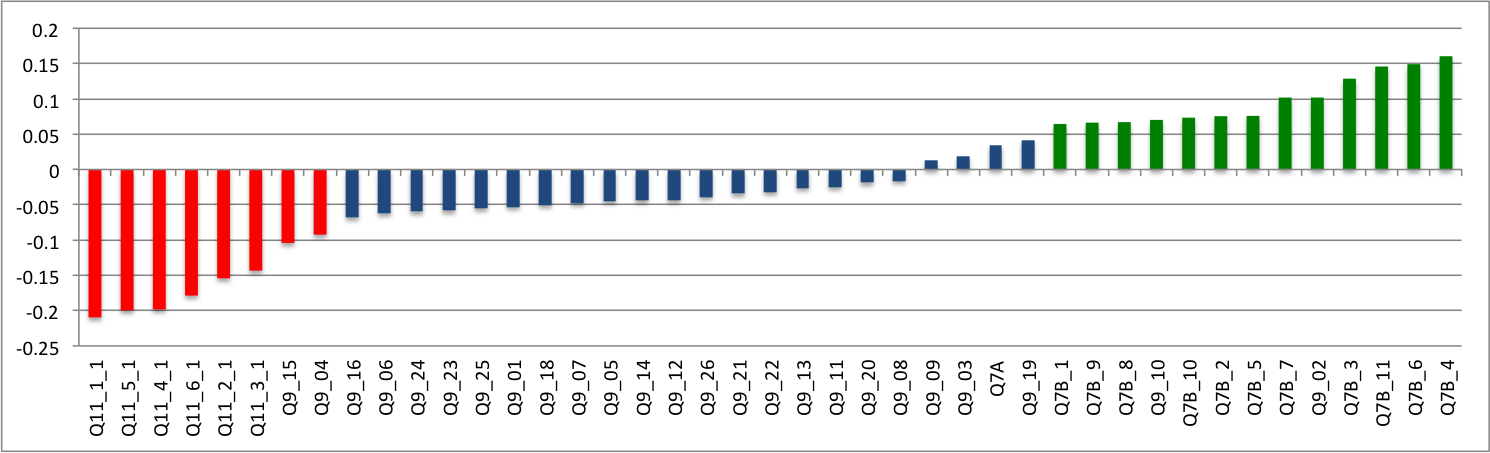
\includegraphics[ width=\textwidth ]{CM1_Cluster6.png}
	\caption{CM1 Scores for the 43 features for Cluster6, based on the new dataset.
	The selected top and bottom features are shown in red and green respectively
	and are presented in Tables~\ref{tab:bottom} and~\ref{tab:top}. The most
	negative ranked features are from question Q11 which suggests a low concern
	about the information may charities provide. On the other hand, the most
	positive positive features are from question Q7B which suggests a higher
	trust and confidence in institutions and organizations.}
	\label{fig:CM1Cluster6}
\end{figure}
\begin{figure}[h]
	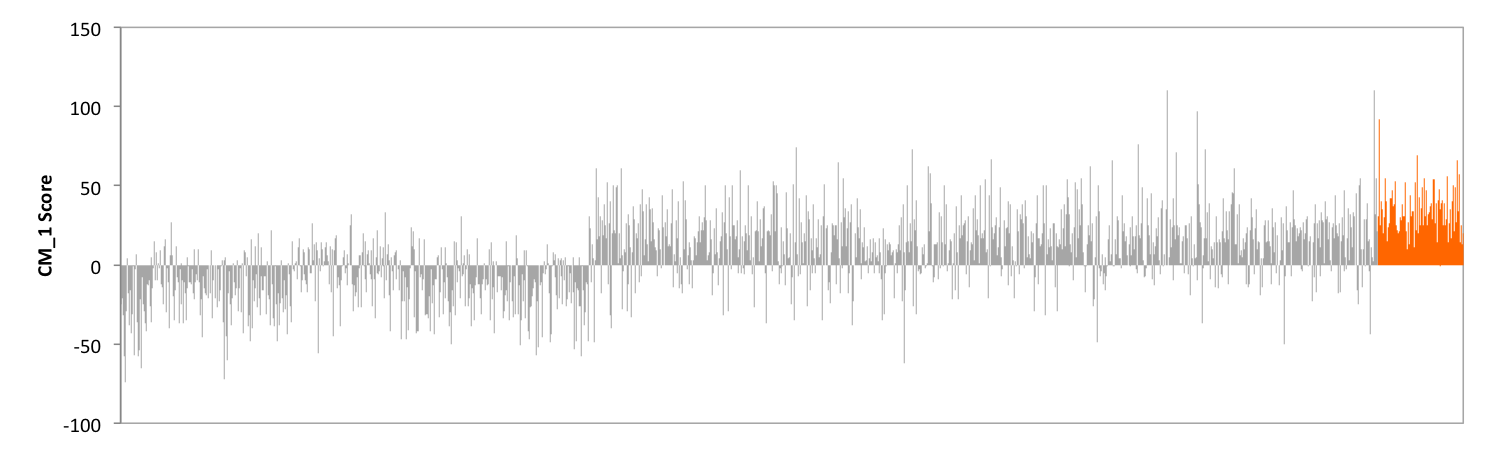
\includegraphics[ width=\textwidth]{Difference_Cluster6.png}
	\caption{Difference between the cumulative CM1 scores for the 8 bottom and 13
	top features for Cluster6, as presented in Tables~\ref{tab:bottom}
	and~\ref{tab:top}. The respondents of Cluster6 are shown in orange. It is
	observed that they score strong positive results against these features}
	\label{fig:DifferencesCluster6}
\end{figure}



\subsubsection{Description of Clusters}


\subsection{Discussion and Conclusion}
%(together)

\bibliography{references}

\end{document}



